\chapter{Getting started}
\label{getting-started}
Systems can be described in \textsc{Line} using one of the available classes of stochastic models:
\begin{itemize}
\item \texttt{Network} models are extended queueing networks. Typical instances are open, closed and mixed queueing networks, including advanced features such as class-switching, finite capacity,
    priorities, non-exponential distributions, and others. Technical background on
    these models can be found in books such as \cite{BolGMT06,LazZGS84} or in tutorials \cite{Lav89,Bal00}.
\item \texttt{LayeredNetwork} models are layered queueing networks, i.e., models consisting of layers, each corresponding
    to a \texttt{Network} object, which interact through synchronous and asynchronous calls. Technical background on
    layered queueing networks can be found in \cite{lqntut}.
%\item \texttt{RandEnv} models describe a system operating in a random environment, i.e., an environment with a state that evolves stochastically. Each state of the environment is associated to a \texttt{Network} object that represents system operation while the environment remains in that state. See \cite{CasTH14} for an introduction.
\end{itemize}
The goal of this chapter is to provide simple examples that explain the basics on how these models can be analyzed in \textsc{Line}. More advanced forms of evaluation, such as probabilistic or transient analyses, are discussed in later chapters. Additional examples are supplied under the \texttt{examples/} folder.

\section{Example 1: A M/M/1 queue}
\label{example-1-mm1-queue}
The M/M/1 queue is a classic model of a queueing system where jobs arrive into an infinite-capacity buffer, wait to be processed by a server in first-come first-served (FCFS) order, and then leave after service completion. Arrival and service times are assumed to be independent and exponentially distributed random variables.

In this example, we wish to compute average performance measures for the M/M/1 queue. We assume that arrivals come in at rate $\lambda=1$ job/s, while service has rate $\mu=2$ job/s. It is known from theory that the exact value of the server utilization then is $\rho=\lambda/\mu=0.5$, i.e., 50\%, while the mean response time for a visit is $R=1/(\mu-\lambda)=1$s. We wish to verify these values using JMT-based simulation, instantiated through \textsc{Line}.

The general structure of a \textsc{Line} script consists of four blocks:
\begin{enumerate}
\item Definition of nodes
\item Definition of job classes and associated statistical distributions
\item Instantiation of model topology
\item Solution
\end{enumerate}
For example, the following script solves the M/M/1 model
\begin{lstlisting}
model = Network('M/M/1');
% Block 1: nodes
source = Source(model, 'mySource');
queue = Queue(model, 'myQueue', SchedStrategy.FCFS);
sink = Sink(model, 'mySink');
% Block 2: classes
oclass = OpenClass(model, 'myClass');
source.setArrival(oclass, Exp(1));
queue.setService(oclass, Exp(2));
% Block 3: topology
model.link(Network.serialRouting(source,queue,sink));
% Block 4: solution
SolverJMT(model,'seed',23000).getAvgTable
\end{lstlisting}
In the example, \texttt{source} and \texttt{sink} are arrival and departure points of jobs; \texttt{oclass} defines an open class of jobs that arrive and leave the system; \texttt{Exp(x)} defines an exponential distribution with rate \texttt{x}; finally, the last command solves for average performance measures with JMT's simulator, using for reproducibility a specific seed for the random number generator.

The result is a table with mean performance measures including: the number of jobs in the station either queueing or receiving service (\texttt{QLen}); the utilization of the servers (\texttt{Util}); the mean response time per visit to the station (\texttt{RespT}); the mean throughput of departing jobs (\texttt{Tput})
\begin{lstlisting}
ans =
  2x6 table
    'mySource'    'myClass'         0          0          0    0.99894
    'myQueue'     'myClass'    0.9555    0.48736    0.95429    0.99987
\end{lstlisting}
One can verify that this matches JMT results by typing
\begin{lstlisting}
model.jsimgView
\end{lstlisting}
which will open the model inside JSIMgraph, as shown in Figure~\ref{FIG:jsimgViewMM1}. From this screen, the simulation can be started using the green ``play'' button in the JSIMgraph toolbar.
\begin{figure}[ht!]
  \centering
  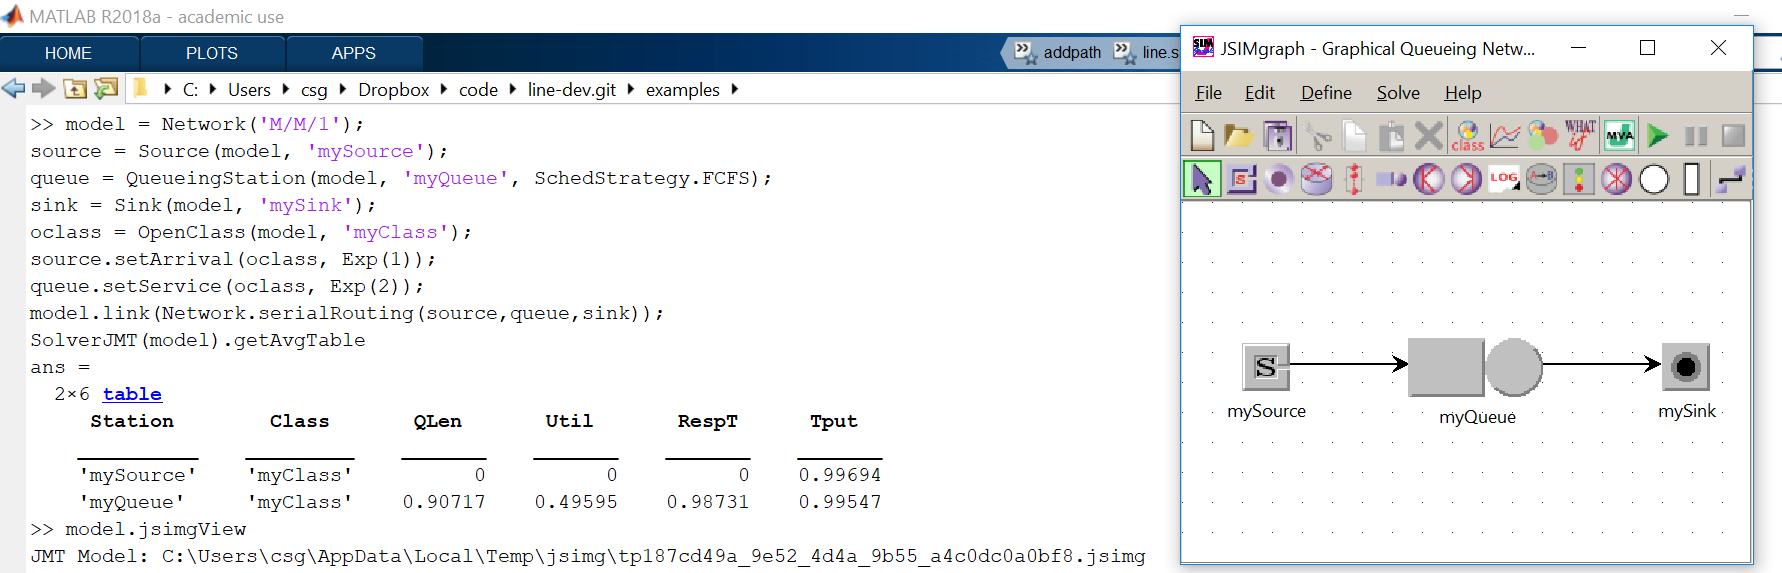
\includegraphics[width=14cm]{./images/jsimgViewMM1.png}
  \caption{M/M/1 example in JSIMgraph}\label{FIG:jsimgViewMM1}
\end{figure}

\section{Example 2: A multiclass M/G/1 queue}
\label{example-2-multiclass-mgk-queue}
We now consider a more challenging variant of the first example. We assume that there are two classes of incoming jobs with non-exponential service times. For the first class, service times are Erlang distributed with unit rate and variance $1/3$; they are instead read from a trace for the second class. Both classes have exponentially distributed service times with mean $2s$. To run this example, we assume that the reader has changed directory in MATLAB to the \texttt{examples/} folder.

We first specify the node block
\begin{lstlisting}
clear;
model = Network('M/G/1');
source = Source(model,'Source');
queue = Queue(model, 'Queue', SchedStrategy.FCFS);
sink = Sink(model,'Sink');
\end{lstlisting}
The next step consists in defining the classes. We fit automatically from mean and squared coefficient of variation (i.e., variance/mean$^2$) an Erlang distribution and use the \texttt{Replayer} distribution to request that the specified trace is cyclically read to obtain the service times of class 2
\begin{lstlisting}
jobclass1 = OpenClass(model, 'Class1');
jobclass2 = OpenClass(model, 'Class2');

source.setArrival(jobclass1, Exp(0.5));
source.setArrival(jobclass2, Exp(0.5));

queue.setService(jobclass1, Erlang.fitMeanAndSCV(1, 1/3));
queue.setService(jobclass2, Replayer('example_trace.txt'));
\end{lstlisting}
Note that the \texttt{example\_trace.txt} file consists of a single column of doubles, each representing a service time sample, e.g.,
\begin{lstlisting}
   1.2377474e-02
   4.4486055e-02
   1.0027642e-02
   2.0983173e-02
   ...
\end{lstlisting}
We now specify a linear route through source, queue, and sink for both classes
\begin{lstlisting}
P = {};
P{jobclass1} = Network.serialRouting(source,queue,sink);
P{jobclass2} = Network.serialRouting(source,queue,sink);
model.link(P);
\end{lstlisting}
and solve the model with JMT
\begin{lstlisting}
>>AvgTable = SolverJMT(model).getAvgTable
AvgTable =
  4x6 table
    Station      Class       QLen        Util       RespT      Tput
    ________    ________    _______    ________    _______    _______
    'Source'    'Class1'          0           0          0     0.5022
    'Source'    'Class2'          0           0          0    0.49999
    'Queue'     'Class1'    0.92002     0.51294     1.7724     0.5071
    'Queue'     'Class2'    0.44506    0.051639    0.85211    0.49996
\end{lstlisting}
We wish now to validate this value against an analytical solver. Since \texttt{jobclass2} has trace-based service times, we first need to revise its service time distribution to make it analytically tractable, e.g., we may ask \textsc{Line} to fit a Cox-2 distribution based on the trace
\begin{lstlisting}
queue.setService(jobclass2, Replayer('example_trace.txt').fitCox());
\end{lstlisting}
We can now use a Continuous Time Markov Chain (CTMC) to solve the system, but since the state space is infinite in open models, we need to truncate it to be able to use this solver. For example, we may restrict to states with at most 2 jobs in each class, checking with the \texttt{verbose} option the size of the resulting state space
\begin{lstlisting}
>> SolverCTMC(model,'cutoff',2,'verbose',true).getAvgTable
State space size: 46 states.
CTMC analysis completed in 0.096734 sec
ans =
  4x6 table
    Station      Class       QLen        Util       RespT      Tput
    ________    ________    _______    ________    _______    _______
    'Source'    'Class1'          0           0          0    0.44948
    'Source'    'Class2'          0           0          0    0.48424
    'Queue'     'Class1'    0.56734     0.44948     1.2863    0.44107
    'Queue'     'Class2'    0.24455    0.048942    0.51396    0.47583
\end{lstlisting}
However, we see from comparison with the JMT results that the errors are rather large. Since the truncated state space consists of just 46 states, we can further increase the cutoff to 4, trading a slower solution time for higher precision
\begin{lstlisting}
>> SolverCTMC(model,'cutoff',4,'verbose',true).getAvgTable
State space size: 626 states.
CTMC analysis completed in 1.051784 sec
ans =
  4x6 table
    Station      Class       QLen        Util       RespT      Tput
    ________    ________    _______    ________    _______    _______
    'Source'    'Class1'          0           0          0    0.49215
    'Source'    'Class2'          0           0          0    0.49626
    'Queue'     'Class1'     0.7958     0.49215     1.6187    0.49162
    'Queue'     'Class2'    0.37558    0.050157    0.75763    0.49573
\end{lstlisting}
To gain more accuracy, we could either keep increasing the cutoff value or, if we wish to compute an exact solution, we may call the matrix-analytic method (MAM) solver instead. MAM uses the repetitive structure of the CTMC to analyze exactly open systems with an infinite state space
\begin{lstlisting}
>> SolverMAM(model).getAvgTable
AvgTable =
  4x6 table
    Station      Class        QLen        Util       RespT      Tput
    ________    ________    ________    ________    _______    _______
    'Source'    'Class1'          0           0          0        0.5
    'Source'    'Class2'          0           0          0        0.5
    'Queue'     'Class1'    0.87646         0.5     1.7529        0.5
    'Queue'     'Class2'      0.427    0.050536    0.85399        0.5
\end{lstlisting}
The current \texttt{MAM} implementation is primarily constructed on top of the BuTools solver~\cite{Hor17}.

\section{Example 3: Machine interference problem}
\label{example-3-machine-interference-problem}
Closed models involve jobs that perpetually cycle within a network of queues. The machine interference problem is a classic example, in which a group of repairmen is tasked with fixing machines as they break and the goal is to choose the optimal size of the group. We here illustrate how to evaluate the performance of a given group size. We consider a scenario with two repairmen, with machines that break at a rate of $4.0$ failed machines/week, after which a machine operates as normal for an exponential distributed time with rate $0.5$ failed machines/week. There are a total of $N=3$ machines.

Suppose that we wish to obtain an exact numerical solution using Continuous Time Markov Chains (CTMCs). The above model can be analyzed as follows:
\begin{lstlisting}
model = Network('MIP');
% Block 1: nodes
delay = Delay(model,'WorkingState');
queue = Queue(model, 'RepairQueue', SchedStrategy.FCFS);
queue.setNumberOfServers(2);
% Block 2: classes
cclass = ClosedClass(model, 'Machines', 3, delay);
delay.setService(cclass, Exp(0.5));
queue.setService(cclass, Exp(4.0));
% Block 3: topology
model.link(Network.serialRouting(delay,queue));
% Block 4: solution
SolverCTMC(model,'keep',true).getAvgTable
\end{lstlisting}
Here, \texttt{delay} appears in the constructor of the closed class to specify that a machine fixing job will be considered completed once it returns to the delay (i.e., the machine is in working state). We say that the delay is thus the \emph{reference station} of class \texttt{cclass}. The above code prints the following result
\begin{lstlisting}
ans =
  2x6 table
       Station          Class        QLen       Util       RespT      Tput
    ______________    __________    _______    _______    _______    ______
    'WorkingState'    'Machines'     2.6648     2.6648          2    1.3324
    'RepairQueue'     'Machines'    0.33516    0.16655    0.25154    1.3324
\end{lstlisting}
As before, we can inspect and analyze the model in JSIMgraph using the command
\begin{lstlisting}
model.jsimgView
\end{lstlisting}
Figure~\ref{FIG:jsimgViewFRP} illustrates the result, demonstrating the automated definition of the closed class.
\begin{figure}[h!t]
  \centering
  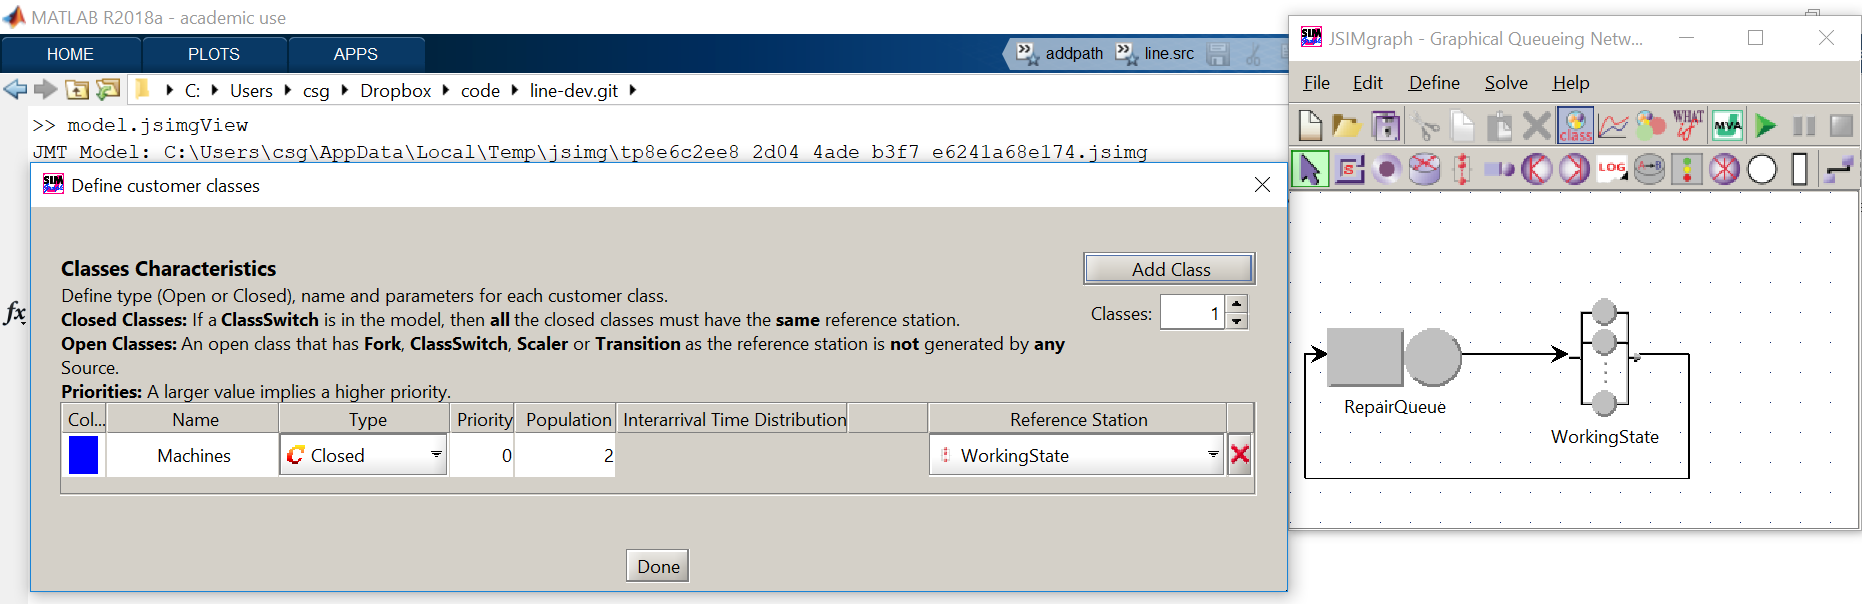
\includegraphics[width=14cm]{./images/jsimgViewFRP.png}
  \caption{Machine interference model in JSIMgraph}\label{FIG:jsimgViewFRP}
\end{figure}

The \texttt{'keep'} option we have used further allows us to inspect the infinitesimal generator of the CTMC. To do so, we retrieve some global variables that have been stored by the CTMC solver, i.e.:
\begin{lstlisting}
global InfGen;
global StateSpace;
StateSpace
InfGen=full(InfGen)
\end{lstlisting}
which produces in output the state space of the model and the infinitesimal generator of the CTMC
\begin{lstlisting}
StateSpace =
     0     1     2
     1     0     2
     2     0     1
     3     0     0
InfGen =
   -8.0000    8.0000         0         0
    0.5000   -8.5000    8.0000         0
         0    1.0000   -5.0000    4.0000
         0         0    1.5000   -1.5000
\end{lstlisting}
For example, the first state (\texttt{0 1 2}) consists of two components: the \texttt{0} is the number of jobs in service in the \texttt{delay}, while the remaining part is the state of the FCFS \texttt{queue}. In the latter, the \texttt{1} means that a job of class 1 (the only class in this model) is in the waiting buffer, while the \texttt{2} means that there are two jobs in service at the \texttt{queue}.

The second state (\texttt{1 0 2}) is similar, but one job has completed at the {queue} and then moved to the \texttt{delay}, concurrently triggering an admission in service for the job that was in the queue buffer. As a result of this, the buffer is now empty. The corresponding transition rate in the infinitesimal generator matrix is \texttt{InfGen(1,2)=8.0}, which sums the completion rates at the queue for each server, and where indexes 1 and 2 are the rows in \texttt{StateSpace} associated to the two states.

\section{Example 4: Round-robin load-balancing}
\label{example-4-round-robin-load-balancing}
In this example we consider a system of two parallel processor-sharing queues and we wish to study the effect of load-balancing on the average performance of an open class of jobs. We begin as usual with the node block, where we now include a special node, called the \texttt{Router}, to control the routing of jobs from the source into the queues:
\begin{lstlisting}
model = Network('RRLB');
source = Source(model, 'Source');
lb = Router(model, 'LB');
queue1 = Queue(model, 'Queue1', SchedStrategy.PS);
queue2 = Queue(model, 'Queue2', SchedStrategy.PS);
sink  = Sink(model, 'Sink');
\end{lstlisting}
We then define the class block by setting exponentially-distributed inter-arrival times and service times, e.g.,
\begin{lstlisting}
oclass = OpenClass(model, 'Class1');
source.setArrival(oclass, Exp(1));
queue1.setService(oclass, Exp(2));
queue2.setService(oclass, Exp(2));
\end{lstlisting}
We now wish to express the fact that the router applies a round-robin strategy to dispatch jobs to the queues. Since this is now a non-probabilistic routing strategy, we need to adopt a slightly different style to declare the topology. First, we indicate the connections between the nodes, using the \texttt{addLinks} function:
\begin{lstlisting}
model.addLinks([source, lb;
                lb,     queue1;
                lb,     queue2;
                queue1, sink;
                queue2, sink]);
\end{lstlisting}
At this point, all nodes are automatically configured to route jobs with equal probabilities on the outgoing links (\texttt{RoutingStrategy.RAND} policy). If we solve the model at this point, we see that the response time at the queues is around $0.66 s$.
\begin{lstlisting}
>> SolverJMT(model).getAvgTable
ans =
  3x6 table
    Station      Class       QLen       Util       RespT      Tput
    ________    ________    _______    _______    _______    _______
    'Source'    'Class1'          0          0          0     1.0178
    'Queue1'    'Class1'    0.32089    0.24179    0.65821    0.50222
    'Queue2'    'Class1'    0.32605    0.25078    0.66978    0.50161
\end{lstlisting}

After resetting the internal data structures, we can require \textsc{Line} to solve again the model using this time a round-robin policy at the router.
\begin{lstlisting}
model.reset()
lb.setRouting(oclass, RoutingStrategy.RR);
\end{lstlisting}
A representation of the model at this point is shown in Figure~\ref{FIG:jsimgViewLB}.
\begin{figure}[h!t]
  \centering
  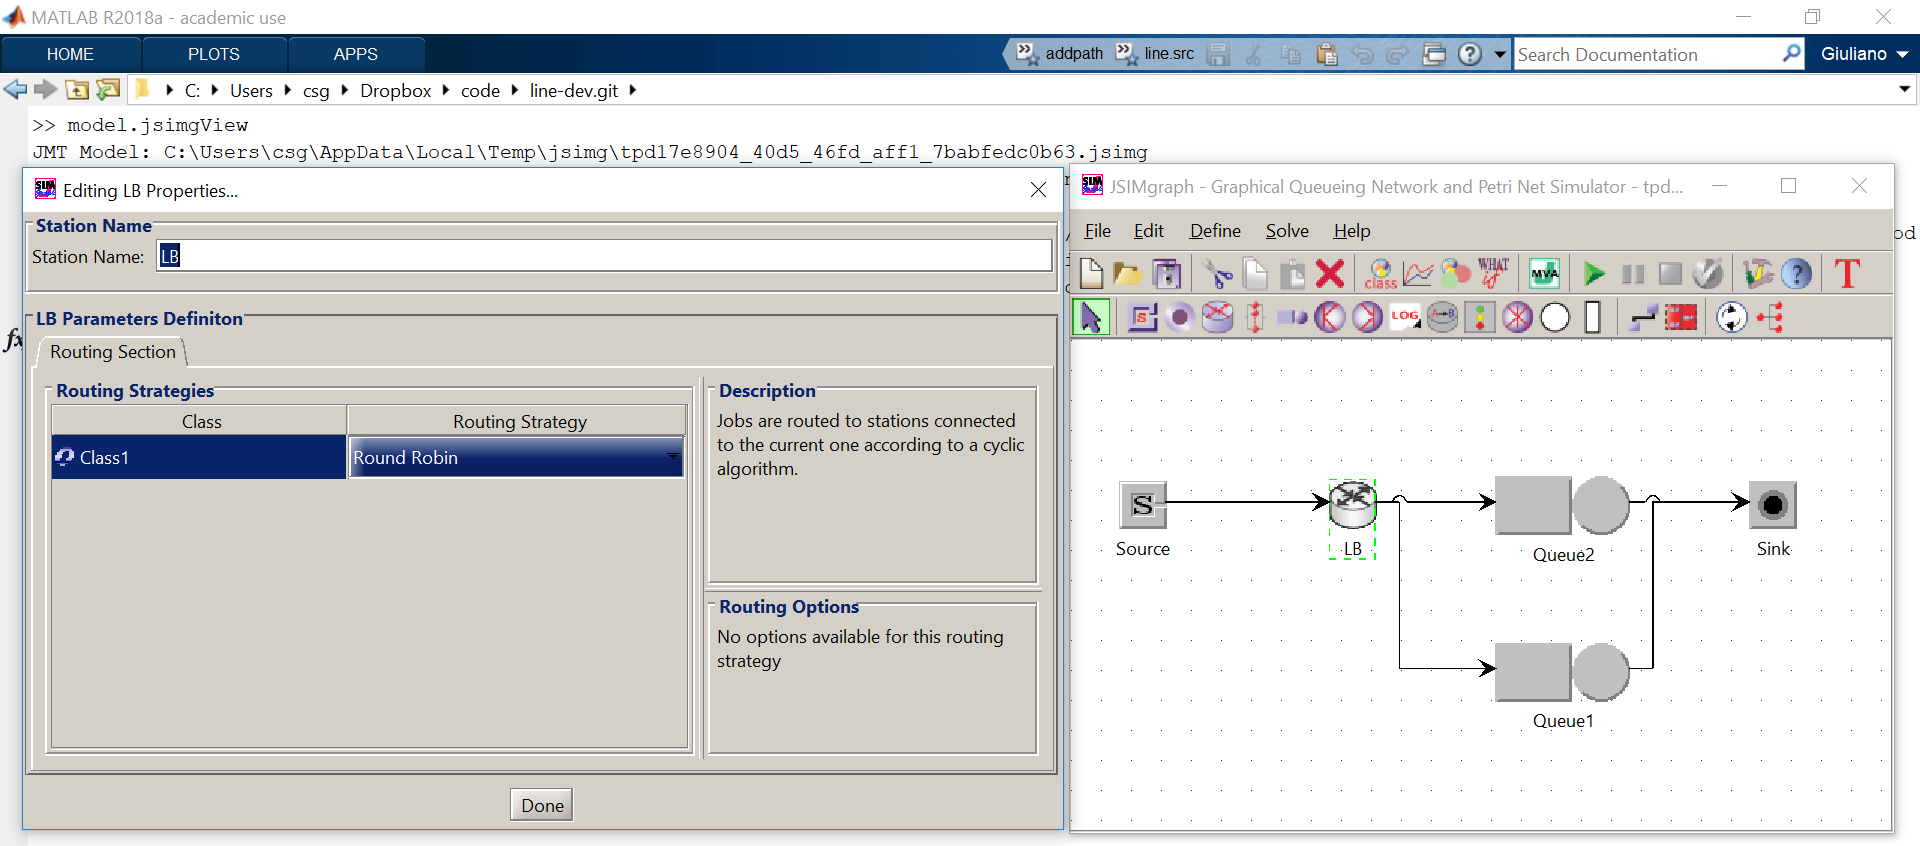
\includegraphics[width=14cm]{./images/jsimgViewLB.png}
  \caption{Load-balancing model}\label{FIG:jsimgViewLB}
\end{figure}
Lastly, we run again JMT and find that round-robin produces a visible decrease in response times
\begin{lstlisting}
>> SolverJMT(model).getAvgTable
  3x6 table
    Station      Class       QLen       Util       RespT      Tput
    ________    ________    _______    _______    _______    _______
    'Source'    'Class1'          0          0          0    0.97298
    'Queue1'    'Class1'    0.27649    0.24399    0.55775    0.48615
    'Queue2'    'Class1'    0.29316    0.24761    0.56565     0.4932
\end{lstlisting}

\section{Example 5: Modelling a re-entrant line}
\label{example-5-modelling-a-re-entrant-line}
We now consider a simple example inspired to the classic problem of modeling {\em re-entrant lines}. This arises in manufacturing systems where parts (i.e., jobs) re-enter multiple times a machine (i.e., a queueing station), asking at every visit a different class of service. This implies, for example, that the service time at every visit could feature a different mean or a different distribution, representing a different stage of processing for the part.

To illustrate this, consider for example a degenerate model composed by a single FCFS queue and $K$ classes. In this model, a job that completes processing in class $k=1,...,K$ is routed back at the tail of the queue in class $k+1$, unless $k=K$ in which case the job re-enters in class $1$.

We take the following assumptions: $K=3$; class $k$ has an Erlang-2 distribution with mean $k$; the system starts with $N_1=1$ jobs in class 1 and no jobs inside the other classes.

\begin{lstlisting}
model = Network('RL');
queue = Queue(model, 'Queue', SchedStrategy.FCFS);

K = 3; N = [1,0,0];
for k=1:K
    jobclass{k} = ClosedClass(model, ['Class',int2str(k)], N(k), queue);
    queue.setService(jobclass{k}, Erlang.fitMeanAndOrder(k,2));
end

P = cellzeros(3,3,1,1); % 3x3 cell array (3 classes) of 1x1 matrices (1 node)
P{jobclass{1},jobclass{2}}(queue,queue) = 1.0;
P{jobclass{2},jobclass{3}}(queue,queue) = 1.0;
P{jobclass{3},jobclass{1}}(queue,queue) = 1.0;
model.link(P);
\end{lstlisting}
The corresponding JMT model is shown in Figure~\ref{FIG:jsimgViewCS}, where it can be seen that the class-switching rule is automatically enforced by introduction of a \texttt{ClassSwitch} node in addition to the queue.
\begin{figure}[h!t]
  \centering
  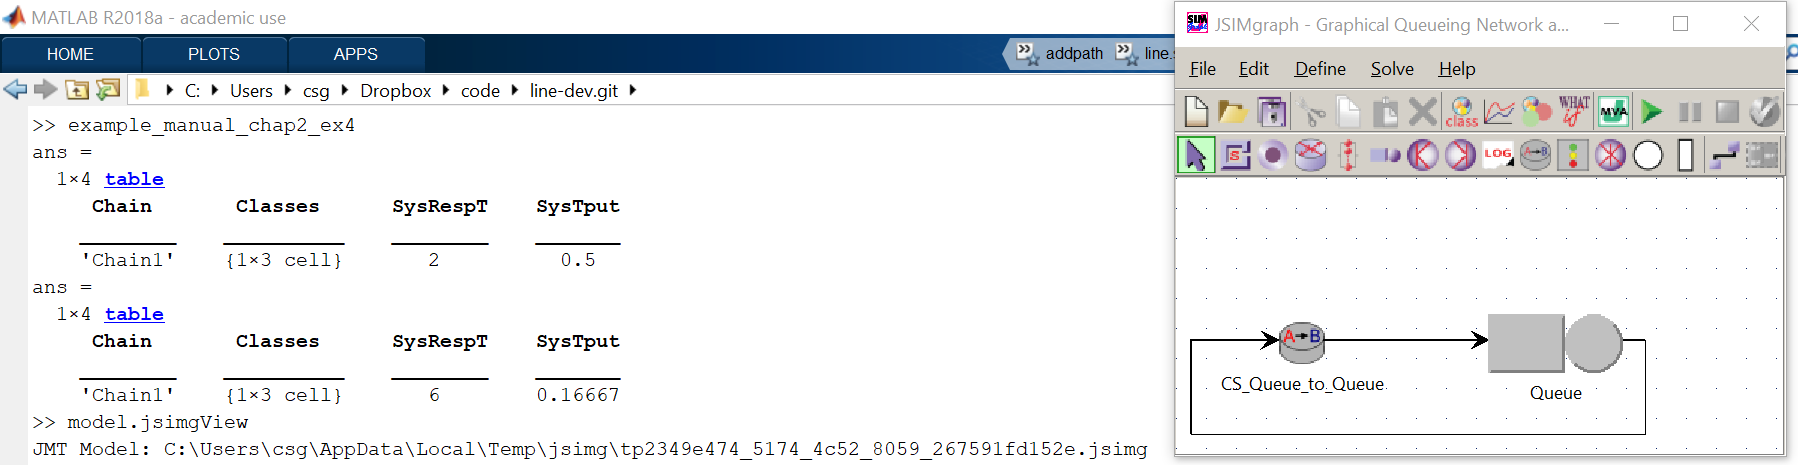
\includegraphics[width=14cm]{./images/jsimgViewCS.png}
  \caption{Re-entrant lines as an example of class-switching}
  \label{FIG:jsimgViewCS}
\end{figure}

We can now simulate the performance indexes for the different classes
\begin{lstlisting}
>> SolverCTMC(model).getAvgTable
ans =
  3x6 table
    Station     Class       QLen       Util      RespT     Tput
    _______    ________    _______    _______    _____    _______
    'Queue'    'Class1'    0.16667    0.16667      1      0.16667
    'Queue'    'Class2'    0.33333    0.33333      2      0.16667
    'Queue'    'Class3'        0.5        0.5      3      0.16667
\end{lstlisting}
Suppose now that the job is considered completed, for the sake of computation of the system's performance, only when it departs the queue in class $K$ (here \texttt{Class3}). By default, \textsc{Line} will return \emph{system-wide} performance metrics using the \texttt{getAvgSysTable} method, i.e.,
\begin{lstlisting}
>> SolverCTMC(model).getAvgSysTable
ans =
  1x4 table
     Chain       Classes      SysRespT    SysTput
    ________    __________    ________    _______
    'Chain1'    {1x3 cell}       2          0.5
\end{lstlisting}
This method identifies the model \emph{chains}, i.e., groups of classes that can exchange jobs with each other. Since the job can switch into any of the three classes, here there is a single chain comprising all three classes.

We see, however, that the throughput of this chain is $0.5$, which means that by default \textsc{Line} is counting every departure from the queue as a completion. This is because in the constructor of the closed classes, we specified \texttt{queue} as the reference station for all three classes. We could have not chosen otherwise as solution algorithms expect that all classes in a chain share the same reference station. 

To avoid this complication, we can explicitly tell to the solver that some passages through the reference station should not be counted as completions
\begin{lstlisting}
jobclass{1}.completes = false;
jobclass{2}.completes = false;
\end{lstlisting}
this then gives the correct throughput
\begin{lstlisting}
>> SolverCTMC(model).getAvgSysTable
ans =
  1x4 table
     Chain       Classes      SysRespT    SysTput
    ________    __________    ________    _______
    'Chain1'    {1x3 cell}       6        0.16667
\end{lstlisting}

\section{Example 6: A queueing network with caching}
\label{example-6-a-queueing-network-with-caching}
In this more advanced example, we show how to include in a queueing network a cache adopting a least-recently used (LRU) replacement policy. Under LRU, upon a cache miss the least-recently accessed item will be discarded to make room for the newly requested item.

We consider a cache with a capacity of 50 items, out of a set of 1000 items. Items are accessed by jobs visiting the cache according to a Zipf-like law with exponent $\alpha=1.4$ and defined over the finite set of items. A client cyclically issues requests for the items, waiting for a reply before issuing the next request. We assume that a cache hit takes on average $0.2ms$ to process, while a cache hit takes $1ms$. We ask for the average request throughput of the system, differentiated across hits and misses.

\paragraph{Node block}
As usual, we begin by defining the nodes. Here a delay node will be used to describe the time spent by the requests in the system, while the cache node will determine hits and misses:
\begin{lstlisting}
model = Network('QNC');
% Block 1: nodes
clientDelay = Delay(model, 'Client');
cacheNode = Cache(model, 'Cache', 1000, 50, ReplacementPolicy.LRU);
cacheDelay = Delay(model, 'CacheDelay');
\end{lstlisting}

\paragraph{Class block}
We define a set of classes to represent the incoming requests (\texttt{clientClass}), cache hits (\texttt{hitClass}) and cache misses (\texttt{missClass}). These classes need to be closed to ensure that there is a single outstanding request from the client at all times:
\begin{lstlisting}
% Block 2: classes
clientClass = ClosedClass(model, 'ClientClass', 1, clientDelay, 0);
hitClass = ClosedClass(model, 'HitClass', 0, clientDelay, 0);
missClass = ClosedClass(model, 'MissClass', 0, clientDelay, 0);
\end{lstlisting}
We then assign the processing times, using the \texttt{Immediate} distribution to ensure that the client issues immediately the request to the cache:
\begin{lstlisting}
clientDelay.setService(clientClass, Immediate());
cacheDelay.setService(hitClass, Exp.fitMean(0.2));
cacheDelay.setService(missClass, Exp.fitMean(1));
\end{lstlisting}
The next step involves specifying that the request uses a Zipf-like distribution to select the item to read from the cache
\begin{lstlisting}
cacheNode.setRead(clientClass, Zipf(1.4,1000));
\end{lstlisting}
Finally, we ask that the job should become of class \texttt{hitClass} after a cache hit, and should become of class \texttt{missClass} after a cache miss:
\begin{lstlisting}
cacheNode.setHitClass(clientClass, hitClass);
cacheNode.setMissClass(clientClass, missClass);
\end{lstlisting}

\paragraph{Topology block}
Next, in the topology block we setup the routing so that the request, which starts in \texttt{clientClass} at the \texttt{clientDelay}, then moves from there to the cache, remaining in \texttt{clientClass}
\begin{lstlisting}
% Block 3: topology
P = cellzeros(3,3,4,4); % 3x3 cell (3 classes) of 4x4 zero matrices (4 nodes)
P{clientClass, clientClass}(clientDelay, cacheNode) = 1.0;
\end{lstlisting}
Internally to the cache, the job will switch its class into either \texttt{hitClass} or \texttt{missClass}. Upon departure in one of these classes, we ask it to join in the same class \texttt{cacheDelay} for further processing
\begin{lstlisting}
P{hitClass, hitClass}(cacheNode, cacheDelay) = 1.0;
P{missClass, missClass}(cacheNode, cacheDelay) = 1.0;
\end{lstlisting}
Lastly, the job returns to \texttt{clientDelay} for completion and start of a new request, which is done by switching its class back to \texttt{clientClass}
\begin{lstlisting}
P{hitClass, clientClass}(cacheDelay, clientDelay) = 1.0;
P{missClass, clientClass}(cacheDelay, clientDelay) = 1.0;
\end{lstlisting}
The above routing strategy is finally applied to the model
\begin{lstlisting}
model.link(P);
\end{lstlisting}

\paragraph{Solution block}
To solve the model, since JMT does not support cache modeling, we use the native MATLAB-based simulation engine provided within \textsc{Line}, the \texttt{SSA} solver:
\begin{lstlisting}
% Block 4: solution
AvgTable = SolverSSA(model,'samples',2e4,'seed',1,'verbose',true).getAvgTable
\end{lstlisting}
The above script produces the following result
\begin{lstlisting}
SSA samples:   20000
SSA analysis completed in 11.902675 sec
AvgTable =
 3x6 table
     Station           Class         QLen       Util      RespT     Tput
   ____________    _____________    _______    _______    _____    _______
   'Client'        'ClientClass'          0          0       0      2.9917
   'CacheDelay'    'HitClass'       0.49108    0.49108     0.2      2.4554
   'CacheDelay'    'MissClass'      0.50892    0.50892       1     0.50892
\end{lstlisting}
The departing flows from the \texttt{CacheDelay} are the miss and hit rates. Thus, the hit rate is $2.4554$ req/ms, while the miss rate is $0.50892$ req/ms, which both include the service times.

Let us now suppose that we wish to verify the result with a longer simulation, for example with 10 times more samples. To this aim, we can use the automatic parallelization of \texttt{SSA} based on MATLAB's \texttt{spmd} construct:
\begin{lstlisting}
SolverSSA(model,'samples',2e4,'seed',1,'method','parallel').getAvgTable
\end{lstlisting}
This gives us a rather similar result, when run on a dual-core machine
\begin{lstlisting}
Starting parallel pool (parpool) using the 'local' profile ...
connected to 2 workers.
AvgTable =
 3x6 table
     Station           Class         QLen      Util     RespT     Tput
   ____________    _____________    ______    ______    _____    ______
   'Client'        'ClientClass'         0         0       0     2.8636
   'CacheDelay'    'HitClass'       0.4709    0.4709     0.2     2.3545
   'CacheDelay'    'MissClass'      0.5291    0.5291       1     0.5291
\end{lstlisting}
The execution time is longer than usual at the first invocation of the parallel solver due to the time needed by MATLAB to bootstrap the parallel pool, in this example around 22 seconds. Successive invocations of parallel SSA normally take much less, with this example around 7 seconds each.

%\section{Example 4: Server breakdown and repair}

%\section{Example 5: A two-layer network}
